\section{Overview}
\label{sec:overview}

\begin{figure}[H]
	\centering
	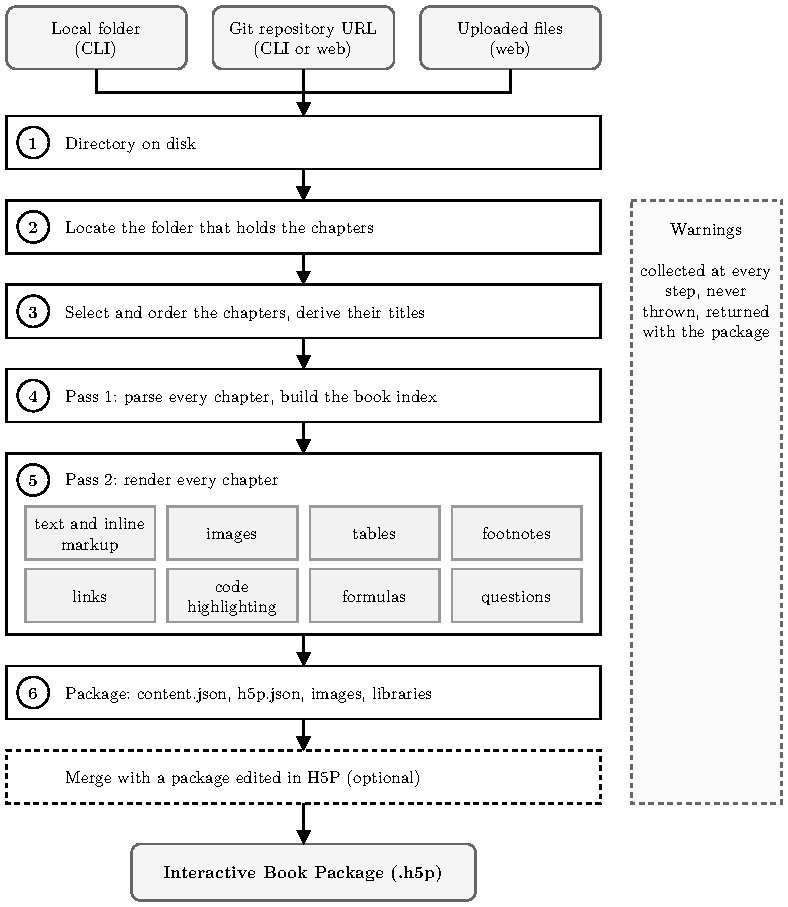
\includegraphics[width=0.92\columnwidth]{figures/pipeline}
	\caption[The conversion pipeline]{\label{fig:pipeline}The conversion pipeline.
	All three input modes produce a directory
		on disk \circled{1}; the folder holding the chapters is located \circled{2}, the chapters are
		selected and ordered \circled{3}, every file is parsed and indexed \circled{4}, then rendered
		\circled{5}, and the result is packaged with the libraries it needs \circled{6}.
		Warnings are
		collected at every step and returned together with the package.}
\end{figure}

The usage examples showed the converter as a black box.
md2h5p is implemented in Kotlin and runs on the Java Virtual Machine (JVM).
This section describes its scope, the steps of a conversion, the three input modes, how errors are
handled, and how an already edited package is updated.
\autoref{fig:pipeline} shows the pipeline; the text refers to its numbered steps.

\paragraph{Scope.}
The converter takes a folder of Markdown files, one per chapter, and produces
an Interactive Book package for Moodle.
It carries over the structure of the text (headings, paragraphs, lists, block quotes), inline
formatting, images, tables, links, footnotes, and code blocks.
It also renders three constructs that go beyond plain Markdown:
highlighted code, formulas, and simple quizzes.
It does not create new H5P content types and does not upload anything to Moodle.
Where Interactive Book cannot represent a construct directly, the converter produces the closest
supported approximation.
Warnings identify input that requires the author's attention.

\paragraph{Pipeline.}
A conversion starts from a directory on disk \circled{1}.
The directory may hold more than the chapters, a whole repository for instance, so the first step
is to find the folder with the Markdown files \circled{2}.
From that folder, they are selected, put into chapter order, and given titles
\circled{3}.
The chapters are then processed in two passes.
The first pass \circled{4} parses every file and records each chapter's title, file name, package identifier,
and heading anchors in an index of the whole book.
The second pass \circled{5} renders each chapter into content blocks, with separate renderers for
the more complex constructs.
Images are resolved and copied during this pass.
Finally, the generated \code{content.json} and \code{h5p.json} are zipped together with the images
and the H5P libraries the book depends on \circled{6}.

This separation into two passes is needed for links.
A link in chapter~2 may point at chapter~5. To render it, the converter has to know whether that
chapter exists, what it is called, and which identifier it carries.
Since a link may point forwards, every chapter has to be parsed before the first one is rendered.

\paragraph{Input Modes.}
The content arrives in one of three ways: a folder on the local machine, a Git repository that is
shallow-cloned, or files uploaded through the browser.
All three end up as a directory on disk \circled{1}, so one pipeline serves every mode.
After that point, the modes differ only in how far the converter trusts the content.
A local folder belongs to the person running the converter, so its Markdown may reference an image
anywhere on that machine.
A clone or an upload, by contrast, was written by somebody else and may only reference files inside its own
directory.

\paragraph{Warnings.}
\label{sec:ov_warnings}
The pipeline does not abort on bad input.
A missing image, a path that leaves the allowed directory, an image format the platform rejects, a
table too wide to be rebuilt around an image, or a quiz without a correct answer each results in a
\emph{warning} and a defined fallback.
The book is still produced, so a single unsupported image in one chapter does not
cost the entire conversion.
The warnings are collected at every step and returned together with the package.
Together, these warnings list what the author has to fix or accept.

\paragraph{Updating an Edited Package.}
Interactive Book can hold content that Markdown cannot express, such as a video or an image with
hotspots, which a teacher adds in the H5P editor after the conversion.
If the Markdown changes afterward, a new conversion would produce a package without these
additions.
The converter therefore accepts the edited package as a second input and merges it with the new
conversion.
The text is rebuilt from the Markdown, while every block added in the editor is kept and placed after
the paragraph it followed before.
The merge is a post-processing step on two finished packages and does not change the pipeline above.
It has two limitations: an edit made in the editor to text that came from Markdown is overwritten,
and when paragraphs are reordered in the Markdown, an added block may end up under the wrong one.
Both cases are reported as warnings.
